\label{chapter_dmd}
In this second chapter, we introduce Dynamic Mode Decomposition (DMD). Firstly, we consider the case of linear dynamical systems and we present two versions of the DMD algorithm: one more similar to the Arnoldi algorithm and one based on the Singular Value Decomposition and more numerically stable. We then analyse in \Cref{section_dmd_arnoldi} the link between the DMD and the Arnoldi algorithm, comparing the three algorithms theoretically and through a toy numerical example. Finally, in \Cref{section_dmd_koopman} we extend DMD to nonlinear dynamics.

\section{Dynamic Mode Decomposition (DMD)}
Let us go back to the case of a linear dynamical system
\begin{equation*}
    \vb{x}_{n+1} = \vb*{A}\vb{x}_n, \qquad \vb*{A}\in\R^{n\times n}.
\end{equation*}
As already discussed, in order to extract the dynamic characteristics we need to analyze the spectral properties of $\vb{A}$. However, in a data-drive perspective, we cannot assume that we have access to $\vb*{A}$, but only to a sequence of snapshots. Therefore, we are interested in computing the eigenpairs of $\vb{A}$, or at least the dominant ones, from a sequence of snapshots
\begin{equation*}
    \label{krylov_space}
    \vb*{V}_1^N = \left[\vb{v}_1, \vb{v}_2, \dots, \vb{v}_N\right] = \left[\vb{v}_1, \vb*{A}\vb{v}_1, \dots, \vb*{A}^N\vb{v}_1\right].
\end{equation*}
Since the columns of $\vb*{V}_1^N$ span a Krylov subspace, it is natural to apply a Krylov subspace method. As we do not have access to the matrix $\vb*{A}$ and we cannot compute products of vectors by this matrix, we cannot directly apply numerically stable algorithms such as the Arnoldi method, and we can rely only on the sequence of snapshots we are given in input. \emph{Dynamic Mode Decomposition} (DMD) \cite{schmid_dynamic_2010} is a variant of the Arnoldi method that does not require computing multiplications by $\vb*{A}$, nor any knowledge of the matrix. 

Let us first suppose that, after a certain number of iterates, we found an $\vb*{A}$-invariant Krylov subspace and that $\vb{v}_N$ can be expressed as a linear combination of the previous linearly independent snapshots, i.e.
\begin{equation}
    \label{vn_exact}
    \vb{v}_N = a_1 \vb{v}_1 + \dots + a_{N-1} \vb{v}_{N-1} = \vb{V}_1^{N-1}\vb{a}, \qquad \vb{a}\in\R^{N-1}.
\end{equation}
We can rewrite the relation in \eqref{vn_exact} as:
\begin{equation*}
    \vb*{A}\vb*{V}_1^{N-1} = \vb*{V}_2^{N} = \vb*{V}_1^{N-1}\vb*{S}
\end{equation*}
where $\vb*{S}$ is the companion matrix associated with $\vb{a}$, defined by:
\begin{equation}
    \label{S_definition}
    \vb*{S} :=
   \begin{bmatrix}
   0     &        &       &      & a_1 \\
   1     & 0      &       &      & a_2 \\
         & \ddots & \ddots&      & \vdots \\ 
         &        & 1     & 0    & a_{N-2} \\
         &        &       & 1    & a_{N-1} \\
   \end{bmatrix}.
\end{equation}
The eigenvalues of $\vb*{S}$ are also eigenvalues of $\vb*{A}$. Indeed, if $\vb*{S}\vb{x} = \lambda \vb{x}, \,\, \vb{x}\neq 0$ then $\vb{y} = \vb{V}_1^{N-1}\vb{x}\neq 0$ (we assumed that the first $N-1$ snapshots are linearly independent) and $\vb*{A}\vb{y} = \vb*{A}\vb{V}_1^{N-1}\vb{x} = \vb{V}_1^{N-1}\vb*{S}\vb{x} = \lambda \vb{V}_1^{N-1}\vb{x} = \lambda \vb{y}$.

In general, $\vb{v}_N$ does not necessarily belong to the Span of the columns of $\vb*{V}_1^{N-1}$, i.e. in general $\vb*{V}_1^{N}$ is non-singular. However, as $N$ increases the snapshots tend to lie in the same direction (or at least in the same subspace) and we can expect that after a critical number of snapshots $\vb{v}_N$ \emph{almost} lies in the $\Span{(\vb*{V}_1^{N-1})}$, i.e. that the angle between $\vb{v}_N$ and $\Span{(\vb*{V}_1^{N-1})}$ is close to zero. Therefore, again assuming that the previous vectors are linearly independent, we we want to write
\begin{equation}
    \label{vn_error}
    \begin{split}
        & \vb{v}_N = a_1 \vb{v}_1 + \dots + a_{N-1} \vb{v}_{N-1} + \vb{r}, \qquad \text{i.e.}\\
        & \vb*{A}\vb*{V}_1^{N-1}  = \vb*{V}_1^{N-1}\vb*{S} + \vb{r}\vb{e}_{N-1}^T
    \end{split}
\end{equation}
so that we minimize the norm of the residual $\vb{r} = \vb{v}_N - \vb*{V}_1^{N-1}\vb{a}$. To solve the corresponding least square problem, we compute the thin QR-decomposition of $\vb*{V}_1^{N-1} = \vb*{Q}\vb*{R}$ and then we obtain
\begin{equation}
    \label{a_qrleastsquare}
    \vb{a} = \vb*{R}^{-1} \vb*{Q}^*\vb{v}_N = (\vb*{V}_1^{N-1})^{\dagger}\vb{v}_N.
\end{equation}
The eigenvalues $\{\lambda_j\}_{j = 1}^{N-1}$ of the companion matrix $\vb*{S}$ are now approximations of the eigenvalues of $\vb*{A}$ and are called \emph{Ritz values}. The corresponding approximate eigenvectors $\vb{y}_j = \vb*{V}_1^{N-1}\vb{x}_j$, where $\vb{x}_j$ is an eigenvector of $\vb*{S}$ are the so called \emph{Ritz vectors}. The following proposition summarizes the properties of the approximations provided by the above described DMD algorithm.

\begin{prop}[\cite{drmac_data_2018}]
Suppose that $\vb*{V}_1^{N-1}$ is of full column rank and let us define the Krylov subspace $\mathcal{V}_k = \range(V_1^k)$ for $k = 1, \dots, N$. Let $\vb{a}$ be computed solving the least square problem 
\begin{equation*}
    \vb{a} = \argmin_{\vb{x}\in\R^{N-1}}\norm{\vb{v}_N - \vb*{V}_1^{N-1}\vb{x}} = (\vb*{V}_1^{N-1})^{\dagger}\vb{v}_N
\end{equation*}
and let $\vb*{S}$ be the companion matrix associated with $\vb{a}$ as in \eqref{S_definition}. Then:
\begin{enumerate}[label=(\roman*)]
    \item $\vb*{S} = (\vb*{V}_1^{N-1})^{\dagger}\vb*{A}\vb*{V}_1^{N-1} = (\vb*{V}_1^{N-1})^{\dagger}\vb*{V}_2^{N}$ is the matrix representation of the projection onto $\mathcal{V}_{N-1}$ of the linear operator defined by $\vb*{A}$ restricted to $\mathcal{V}_{N-1}$, i.e. $P_{\mathcal{V}_{N-1}}\vb*{A}\rvert_{\mathcal{V}_{N-1}}$, in the Krylov basis $\vb*{V}_1^{N-1}$ of  $\mathcal{V}_{N-1}$.
    \item if $\vb{r} = \vb{v}_N - \vb*{V}_1^{N-1}\vb{a} = 0$ then $\vb*{A}\vb*{V}_1^{N-1}  = \vb*{V}_1^{N-1}\vb*{S}$, and each eigenpair $(\lambda, \vb{x})$ of $\vb*{S}$ yields an eigenpair of $\vb*{A}$, $(\lambda, \vb{y} = \vb*{V}_1^{N-1}\vb{x})$ 
    \item if $\vb{r} = \vb{v}_N - \vb*{V}_1^{N-1}\vb{a} \neq 0$ then $\vb*{A}\vb*{V}_1^{N-1}  = \vb*{V}_1^{N-1}\vb*{S} + \vb{r}\vb{e}_{N-1}^T$ and the residual $\vb{r}$ is orthogonal to $\range(\vb*{V}_1^{N-1})$. Moreover each eigenpair $(\lambda, \vb{x})$ of $\vb*{S}$ yields an approximate eigenpair of $\vb*{A}$, $(\lambda, \vb{y} = \vb*{V}_1^{N-1}\vb{x})$ called Ritz pair.
    \item The Ritz pair is an exact eigenpair of the perturbed matrix 
    \begin{equation}
        \label{delta_def}
        \vb*{A} + \vb*{\Delta A}, \qquad \vb*{\Delta A} = - \vb{r}\vb{e}_{N-1}^T (\vb*{V}_1^{N-1})^{\dagger}
    \end{equation}
    \item if $\vb*{A}$ is diagonalizable with eigenvalues $\lambda_1, \dots, \lambda_d$ and eigenvector matrix $\vb*{M}$, then for each eigenvalue $\lambda$ of $\vb*{S}$ it holds
    \begin{equation*}
    \begin{split}
        \min_{\lambda_i}\abs{\lambda - \lambda_i} &\leq \kappa_2(\vb*{M})\norm{\vb*{\Delta A}}_2 \\
        \min_{\lambda_i}\frac{\abs{\lambda - \lambda_i}}{\abs{\lambda_i}} &\leq \kappa_2(\vb*{M})\norm{\vb*{A}^{-1}\vb*{\Delta A}}_2 \text{if $\vb*{A}$ is non-singular}
    \end{split}
    \end{equation*}
    where $\kappa_2(\vb*{M}) = \norm{\vb*{M}}_2\norm{\vb*{M}^{-1}}_2$ is the condition number in $2$-norm of the matrix $\vb*{M}$.
\end{enumerate} 
\end{prop}
\begin{proof}
Since $\vb*{V}_1^{N-1}$ is of full column rank, then $(\vb*{V}_1^{N-1})^{\dagger} = ((\vb*{V}_1^{N-1})^{*}\vb*{V}_1^{N-1})^{-1}(\vb*{V}_1^{N-1})^{*}$ is the matrix representation of the projection onto $\mathcal{V}_{N-1}$ with input basis the canonical basis and output basis $\vb*{V}_1^{N-1}$. Moreover $\vb*{A}\vb*{V}_1^{N-1} = \vb*{V}_2^{N}$ is the matrix representation of the linear operator defined by $\vb*{A}$ restricted to $\mathcal{V}_{N-1}$, whit input basis $\mathcal{V}_{N-1}$ and output basis the canonical basis. Statement $(i)$ follows by composition.

We have already discussed $(ii)-(iii)$ and we know that $\vb*{A}\vb*{V}_1^{N-1}  = \vb*{V}_1^{N-1}\vb*{S} + \vb{r}\vb{e}_{N-1}^T$. Moreover, since $\vb*{V}_1^{N-1}$ is of full column rank $(\vb*{V}_1^{N-1})^{\dagger}\vb*{V}_1^{N-1} = \vb*{I}_{N-1}$, hence :
\begin{equation*}
    \vb*{V}_1^{N-1}\vb*{S} = \vb*{A}\vb*{V}_1^{N-1} - \vb{r}\vb{e}_{N-1}^T = \vb*{A}\vb*{V}_1^{N-1} - \vb{r}\vb{e}_{N-1}^T (\vb*{V}_1^{N-1})^{\dagger}\vb*{V}_1^{N-1}  = (\vb*{A} + \vb*{\Delta A})\vb*{V}_1^{N-1} 
\end{equation*}
and statement $(iv)$ follows. Finally, applying the Bauer-Fike theorem \cite{golub_matrix_2013} the first bound in $(v)$ follows immediately. For the second bound, observe that if $\vb*{A}$ is non singular we can multiply by $\vb*{A}^{-1}$ the equality $(\vb*{A} + \vb*{\Delta A})\vb{x} = \lambda \vb{x}$, obtaining $(\lambda \vb*{A}^{-1}  - \vb*{A}^{-1}\vb*{\Delta A})\vb{x} = \vb{x}$. Hence from the Bauer-Fike theorem:
\begin{equation*}
    \min_{\lambda_i}\abs{1 - \frac{\lambda}{\lambda_i}} = \min_{\lambda_i}\frac{\abs{\lambda - \lambda_i}}{\abs{\lambda_i}} \leq  \kappa_2(\vb*{M}^{-1})\norm{\vb*{A}^{-1}\vb*{\Delta A}}_2 = \kappa_2(\vb*{M})\norm{\vb*{A}^{-1}\vb*{\Delta A}}_2
\end{equation*}
\end{proof}

\section{SVD-based DMD}
The above mentioned method was the original version of the DMD \cite{schmid_dynamic_2010}. However, even if it mathematically correct and equivalent to the Arnoldi method in exact arithmetic (see \Cref{section_dmd_arnoldi}), an implementation using the companion matrix $\vb*{S}$ gives rise to a numerically unstable algorithm that is usually not capable to extract more than one or two dominant eigenpairs. Indeed, as already pointed out, the matrix $\vb*{V}_1^{N-1}$ might be numerically rank deficient, hence ill conditioned. Therefore, even when a QR-factorization $\vb*{V}_1^{N-1} = \vb*{Q}\vb*{R}$ is available, it is not advised to compute $\vb{a}$ as $\vb{a} = \vb*{R}^{-1}\vb*{Q}\vb{v}_N$ or $\vb*{S}$ as $\vb*{S} = \vb*{R}^{-1}\vb*{Q}\vb*{A}\vb*{V}_1^{N-1}$. 

Using the Singular Value Decomposition (SVD) it is possible to obtain a mathematically equivalent but better-conditioned algorithm, which is particularly useful when $\vb*{V}_1^{N-1}$ is close to singular (it is very likely to happen for large $N$). This second version of the DMD is what nowadays is referred as DMD. Suppose that we computed a SVD of the snapshots matrix
\begin{equation*}
    \vb*{V}_1^{N-1} = \vb*{U}\vb*{\Sigma}\vb*{W}^* \qquad \vb*{\Sigma}\in\R^{N-1\times N-1},
\end{equation*}
we can now rewrite \eqref{vn_error} as
\begin{equation}
    \label{vn_error_rewritten}
    \vb*{A}\vb*{U}\vb*{\Sigma}\vb*{W}^* = \vb*{U}\vb*{\Sigma}\vb*{W}^*\vb*{S} + \vb{r}\vb{e}_{N-1}^T = \vb*{V}_2^N
\end{equation}
and rearranging
\begin{equation}
    \label{S_tilde_definition}
    \vb*{U}^*\vb*{A}\vb*{U} = \vb*{U}^*\vb*{V}_2^N\vb*{W}\vb*{\Sigma}^{-1} =: \widetilde{\vb*{S}}.
\end{equation}
Once we have computed the eigenpairs $\{(\lambda_j, \vb{x}_j)\}_j$ of the matrix $\widetilde{\vb*{S}}$, which in this case is a full matrix and not of companion type, we obtain the Ritz values and vectors as $\{(\lambda_j, \vb*{U}\vb{x}_j)\}_j$. 

Besides the better conditioning, a great advantage of the SVD-based approach over the Arnoldi-based one is the opportunity to account for rank deficiency in $\vb*{V}_1^{N-1}$ and noise in the data by truncating the SVD of $\vb*{V}_1^{N-1}$. Indeed, we might include a first step in which the matrix $\vb*{V}_1^{N-1}$ is approximated by a low-rank matrix with approximately the same \emph{numerical} rank. This is achieved in a standard way, that is truncating the SVD of the matrix $\vb*{V}_1^{N-1}$ as suggested by the Eckhart–Young-Mirsky theorem \cite{golub_matrix_2013}. The use of TSVD can be particularly useful when using data from experiments, as the problem might be ill-conditioned. 

As previously mentioned, the two approaches are equivalent since $\vb*{S}$ and $\widetilde{\vb*{S}}$ are linked through a similarity transformation, as long as $\vb*{V}_1^{N-1}$ is of full column rank and we do not truncate the SVD. This is summarized in the following proposition
\begin{prop}
\label{prop_svd_dmd}
Suppose that $\vb*{V}_1^{N-1}$ is of full column rank and let $\vb*{V}_1^{N-1} = \vb*{U}\vb*{\Sigma}\vb*{W}^{*}$ be its SVD. Given $k\in\{1,2,\dots, N-1\}$, let us define $\vb*{U}_k = \vb*{U}(\,:\,, 1:k)$, $\vb*{W}_k = \vb*{W}(\,:\,, 1:k)$, $\vb*{\Sigma}_k = \vb*{\Sigma}(1:k, 1:k)$ and finally $\widetilde{\vb*{S}} = \vb*{U}_k^*\vb*{V}_2^N\vb*{W}_k\vb*{\Sigma}_k^{-1}$. Then:
\begin{enumerate}[label=(\roman*)]
    \item if $k = N-1$, i.e. if we do not truncate the SVD, then $\widetilde{\vb*{S}}$ is similar to $\vb*{S}$, where $\vb*{S}$ is defined as in \eqref{S_definition} and the similarity is realized by the matrix $\vb*{W}\vb*{\Sigma}^{-1}$.
    \item if $k < N-1$, then $\widetilde{\vb*{S}}$ is the matrix representation in the basis $\vb*{W}_k\vb*{\Sigma}^{-1}_k$ of the projection onto $\range(\vb*{W}_l\vb*{\Sigma}^{-1}_k)$ of the linear operator defined by $\vb*{S}$ restricted to $\range(\vb*{W}_k\vb*{\Sigma}^{-1}_k)$.
    \item $\widetilde{\vb*{S}}$ is the matrix representation in the basis $\vb*{U}_k$ of the projection onto $\range(\vb*{U}_k)$ of the linear operator defined by $\vb*{A}$ restricted to $\range(\vb*{U}_k)$.
\end{enumerate}
\end{prop}
\begin{proof}
Let us first suppose that $k=m$, i.e. that the SVD is not truncated. Then the residual of the least squares solution is orthogonal to the columns of $\vb*{U}$, hence from \eqref{vn_error_rewritten} and \eqref{S_tilde_definition}:
\begin{equation*}
    \begin{split}
    \widetilde{\vb*{S}} & =
    \vb*{U}^*\vb*{V}_2^N\vb*{W}\vb*{\Sigma}^{-1} =
    \vb*{U}^*(\vb*{U}\vb*{\Sigma}\vb*{W}^*\vb*{S} + \vb{r}\vb{e}_{N-1}^T)\vb*{W}\vb*{\Sigma}^{-1} = \\
    & = (\vb*{\Sigma}\vb*{W}^*) \vb*{S} (\vb*{W}\vb*{\Sigma}^{-1}) =
    (\vb*{W}\vb*{\Sigma}^{-1})^{-1} \vb*{S} (\vb*{W}\vb*{\Sigma}^{-1})    
    \end{split}
\end{equation*}
and the matrices $\widetilde{\vb*{S}}$ and $\vb*{S}$ are liked by the stated similarity transformation.

If $k < m$ we can write $\vb*{V}_1^{N-1} ={ \vb*{U}_k\vb*{\Sigma}_k\vb*{W}^{*}_k + \vb*{\delta V}}$, where $\vb*{\delta V} = {\sum_{i = k+1}^{N-1}\sigma_i\vb*{U}(\,:\,, i)\vb*{W}(\,:\,, i)^*}$ is such that $\vb*{U}_k^{*}\vb*{\delta V} = \vb*{\delta V}\vb*{W}_k = \vb*{0}$. Hence we can write \eqref{vn_error} as
\begin{equation*}
    \vb*{A}(\vb*{U}_k\vb*{\Sigma}_k\vb*{W}^{*}_k + \vb*{\delta V}) = (\vb*{U}_k\vb*{\Sigma}_k\vb*{W}^{*}_k + \vb*{\delta V})\vb*{S} + \vb{r}\vb{e}_{N-1}^T = \vb*{V}_2^N
\end{equation*}
Multiplying by $\vb*{U}_k^*$ on the left and by $\vb*{W}_k\vb*{\Sigma}_k^{-1}$ on the right, we get
\begin{equation*}
    \vb*{U}_k^{*}\vb*{A}\vb*{U}_k = (\vb*{W}_k\vb*{\Sigma}^{-1}_k)^{-1} \vb*{S} (\vb*{W}_k\vb*{\Sigma}^{-1}_k) = \widetilde{\vb*{S}} 
\end{equation*}
and the thesis follows.
\end{proof}

The SVD-based version of DMD is summarized in \Cref{alg_dmd}.

\begin{algorithm}
\caption{\textbf{: SVD-based DMD}}
\label{alg_dmd}
\textbf{Input:} $\vb{v}_1,\dots, \vb{v}_N$
\begin{algorithmic}[1]
\State Define the matrices $\vb*{V}_1^{N-1} = \left[\vb{v}_1,\dots,\vb{v}_{N-1}\right]$ and $\vb*{V}_2^{N} = \left[\vb{v}_2,\dots,\vb{v}_{N}\right]$.
\State Compute the (possibly truncated) SVD of $\vb*{V}_1^{N-1} = \vb*{U}\vb*{\Sigma}\vb*{W}^*,\,\, \vb*{\Sigma}\in\R^{p\times p}$.
\State Define the matrix $\widetilde{\vb*{S}} := \vb*{U}^*\vb*{V}_2^N\vb*{W}\vb*{\Sigma}^{-1}$.
\State Compute the eigenpairs $\{(\lambda_j, \vb{x}_j)\}_j$ of $\widetilde{\vb*{S}}$.
\State Compute the Ritz vector corresponding to the Ritz value $\lambda_j$ as $\vb{y}_j = \vb*{U}\vb{x}_j$. 
\end{algorithmic}
\textbf{Output:} Ritz values $\lambda_1,\dots,\lambda_{p}$ and corresponding Ritz vectors $\vb{y}_1,\dots, \vb{y}_p$
\end{algorithm}

\section{DMD and the Arnoldi method}
\label{section_dmd_arnoldi}
The Arnoldi method and the DMD are equivalent in exact arithmetic. In the following section, we will discuss and prove this statement, emphasizing why the Arnoldi algorithm is generally more stable.

The Arnoldi method computes an orthonormal basis of the Krylov subspace spanned by the columns of $\vb*{V}_1^{N-1}$ computing the snapshots implicitly. In particular, if $\vb*{V}_1^{N-1}$ is of full colum rank and therefore the algorithms does not stop, it computes a matrix $\vb*{Q}_{N-1} = \left[\vb{q}_1,\dots, \vb{q}_{N-1}\right]$ with columns that form an orthonormal basis of $\Span{(\vb*{V}_1^{N-1})}$ and: 
\begin{enumerate}[label=(\roman*)]
    \item $\vb*{V}_1^{N-1} = \vb*{Q}_{N-1} \vb*{R}_{N-1}$ is a thin QR-decomposition (with $\vb*{R}_{N-1}$ that is computed implicitly);
    \item $\vb*{H}_{N-1} = \vb*{Q}_{N-1}^* \vb*{A} \vb*{Q}_{N-1}$ is a Hessenberg matrix.
\end{enumerate}
Then the eigenpairs approximations are obtained from the eigenpairs of $\vb*{H}_{N-1}$. This is mathematically equivalent to the DMD algorithm, as specified in the following proposition. 

\begin{prop}
Suppose that $\vb*{V}_1^{N-1}$ is of full column rank. Then the Arnoldi method and the DMD algorithms are equivalent in exact arithmetic, i.e. the Ritz pairs returned by the two algorithms coincide. 
\end{prop}
\begin{proof}
From \eqref{vn_error} and \eqref{a_qrleastsquare} the residual $\vb{r}$ can be written as
\begin{equation*}
    \vb{r} = \vb{v}_N - \vb*{V}_1^{N-1}\vb*{R}_{N-1}^{-1}\vb*{Q}_{N-1}^*\vb{v}_N = \vb{v}_N - \vb*{Q}_{N-1}\vb*{Q}_{N-1}^*\vb{v}_N
\end{equation*}
and therefore $\vb*{Q}_{N-1}^*\vb{r} = \vb*{0}$.Plugging the QR-decomposition into \eqref{vn_error}
\begin{equation*}
    \vb*{A}\vb*{Q}_{N-1}\vb*{R}_{N-1} = \vb*{Q}_{N-1}\vb*{R}_{N-1}\vb*{S} + \vb{r}\vb{e}_{N-1}^T
\end{equation*}
and multiplying by $\vb*{Q}_{N-1}^*$ on the left and by $\vb*{R}_{N-1}^{-1}$ on the right
\begin{equation}
    \label{similarity_arnoldi_dmd}
    \vb*{H}_{N-1} = \vb*{Q}_{N-1}\vb*{A}\vb*{Q}_{N-1} = \vb*{R}_{N-1}\vb*{S}\vb*{R}_{N-1}^{-1}.
\end{equation}
Hence $\vb*{H}_{N-1}$ and $\vb*{S}$ are linked through a similarity transformation and, in particular, have the same eigenvalues. As a consequence of \Cref{prop_svd_dmd}, this is true also if we apply the SVD-based DMD without truncation.

Let $\vb*{M}_{N-1}$ be eigenvector matrix of $\vb*{H}_{N-1}$, then the Ritz vectors returned by the Arnoldi method are the columns of $\vb*{Q}_{N-1}\vb*{M}_{N-1}$. From \eqref{similarity_arnoldi_dmd}, the eigenvector matrix of $\vb*{S}$ is $\vb*{R}_{N-1}^{-1}\vb*{M}_{N-1}$, thus the Ritz vectors returned by the DMD algorithm are the columns of $\vb*{V}_1^{N-1}\vb*{R}_{N-1}^{-1}\vb*{M}_{N-1} = \vb*{Q}_{N-1}\vb*{R}_{N-1}\vb*{R}_{N-1}^{-1}\vb*{M}_{N-1} = \vb*{Q}_{N-1}^{-1}\vb*{M}_{N-1}$ and also the Ritz vectors coincide.
\end{proof}


Although the two algorithms are equivalent mathematically and in exact arithmetic, the Arnoldi algorithm is numerically more stable. Indeed, as the number of snapshots increases, the vectors tend to become linearly dependent and therefore, the matrix $V_1^N$ becomes close to singular, hence ill-conditioned. Even if the problem can be partially solved using the SVD-based DMD and performing a truncated SVD, another major problem is intrinsic to the data-driven approach. One of the major strengths of the Arnoldi algorithm is that it does not even compute the vectors $\vb{x}_j = \vb*{A}^j \vb{x}_0$ because errors are already made in these computations. However, in a data-driven perspective, this is not possible since what we are given is a sequence of snapshots and not the matrix $\vb*{A}$. Hence, we trade-off better stability and convergence properties for an algorithm that only relies on $V_1^N$ and is therefore applicable to snapshots experimentally collected.

To compare numerically the algorithms, we performed 60 iterations with the matrix \texttt{A} of size \texttt{n = 400} defined as \texttt{A = diag([1, 0.9, 0.8.\^{}(1:n-2)])} and random starting vector \texttt{x = rand(n,1)} normalized. \Cref{fig_arnoldi_vs_DMD} shows the convergence of the approximations of the five dominant eigenvalues. It can be seen that the Arnoldi method is able to approximate all of them up to the epsilon-machine-precision. The Arnoldi-based DMD approximates the first two dominant eigenvalues with an accuracy that is eight orders of magnitude lower than the one obtained with the SVD-based DMD. Moreover, it fails in approximating the remaining 3 eigenvalues. The SVD-based DMD is able to approximate all five dominant eigenvalues, with an accuracy than is lower than the one of the Arnoldi algorithm, but still acceptable. 
\begin{figure}[h]
    \centering
    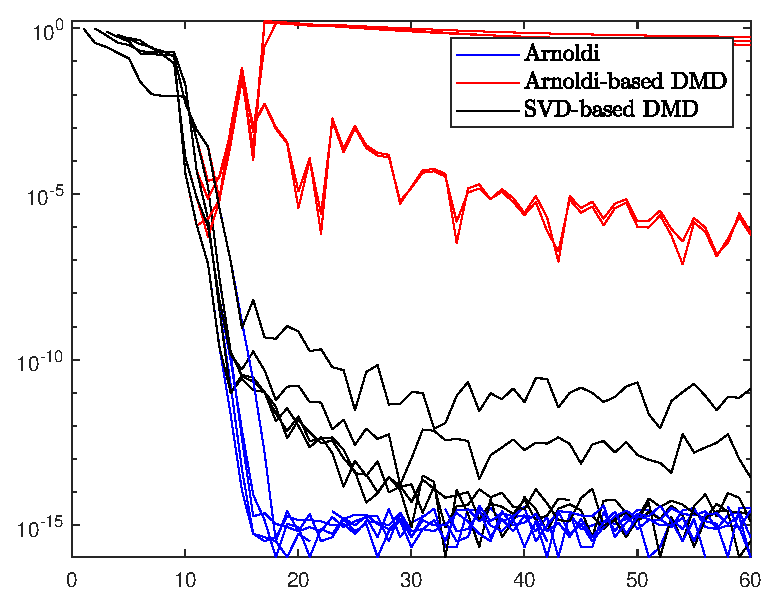
\includegraphics[width=0.5\linewidth]{../code/figures/Arnoldi_vs_DMD.eps}
    \caption{Convergence of the five dominant eigenvalues for the Arnoldi method, the Arnoldi-based DMD algorithm and the SVD-based DMD algorithm. 60 iterations are performed with the matrix \texttt{A} of size \texttt{n = 400} defined as \texttt{A = diag([1, 0.9, 0.8.\^{}(1:n-2)])}.}
    \label{fig_arnoldi_vs_DMD}
\end{figure}

\section{DMD for snapshot data}
\label{section_dmd_koopman}
The original version of the DMD algorithm \cite{schmid_dynamic_2010} assumes that data consist of a trajectory of snapshots $\vb{v}_1, \dots, \vb{v}_N$ where $\vb{v}_{i+1} = \vb*{A}\vb{v}_{i}$. While this is required to write \Cref{vn_error} with $\vb{S}$ a companion matrix, the SVD-based approach does not exploit this structure. Indeed, as observed in \cite{tu_dynamic_2014}, \Cref{alg_dmd} can be carried out for general matrices $\vb*{X}_0$ and $\vb*{X}_1$ replacing $\vb*{V}_1^{N-1}$ and $\vb*{V}_2^{N}$ respectively, where we may assume that
\begin{equation}
    \label{dmd_matrices}
    \vb*{X}_0 = \left[\vb{x}_0^{(1)}, \dots, \vb{x}_0^{(M)}\right] \qquad \vb*{X}_1 = \left[\vb{x}_1^{(1)}, \dots, \vb{x}_1^{(M)}\right]
\end{equation}
are such that $\vb{x}_1^{(m)} = \mathbb{A}\vb{x}_0^{(m)}$ for some linear operator $\mathbb{A}$. This allows to generalise DMD to the case of nonlinear dynamics.

Again, let us start with the linear case, and suppose that instead of snapshots along a single trajectory $\vb{v}_1, \vb{v}_2, \dots, \vb{v}_N$ we are given snapshot pairs of the system state, $\{(\vb{x}_0^{(m)}, \vb{x}_1^{(m)})\}_{m = 1}^M$ with $\vb{x}_1^{(m)} = \vb{F}(\vb{x}_0^{(m)}) = \vb*{A}\vb{x}_0^{(m)}$. The first setting is just a particular case of the latter one, with $\vb{x}_0^{(m)} = \vb{v}_m,\,\,\vb{x}_1^{(m)} = \vb{v}_{m+1}$. However, even in the linear case, requiring in input only snapshot pairs instead of one trajectory allows us to explore as many different initial states as we want. This is of particular help if the trajectories tend to converge to an equilibrium. Let us consider $\vb*{X}_0$ and $\vb*{X}_1$ defined as in \eqref{dmd_matrices}, then the best approximation of $A$ that we can get from data is the least-squares solution is $\hat{\vb*{A}} = \vb*{X}_1\vb*{X}_0^{\dagger}$. The eigenvalues of $\vb*{A}$ can now be approximated by the eigenvalues of $\hat{\vb*{A}}$. The DMD eigenvalues and modes are defined as the nonzero eigenvalues and corresponding eigenvectors of $\hat{\vb*{A}}$, respectively.

If the system is nonlinear, then $\hat{\vb*{A}}$ only provides the best-fit linear approximation of $\vb{F}$, but there is no apparent reason why $\vb{F}$ should be well approximated by a linear finite-dimensional operator. However, even if the dynamics is nonlinear the Koopman Operator is linear (but infinite dimensional). Therefore, we could apply the DMD algorithm to observables in order to obtain an approximation of the Koopman eigenvalues and modes. Let us consider a vector-valued observable $\vb{g} = \vb{g}(\vb{x})$ and its measurements over a set of arbitrary initial states $\{\vb{x}_1,\dots, \vb{x}_M\}$ and one step after. Let us define:
\begin{equation}
    \label{dmd_koopman_matrices}
    \begin{split}
        \vb*{G}_0 &= \left[\vb{g}(\vb{x}_1), \dots, \vb{g}(\vb{x}_M)\right] \\
        \vb*{G}_1 &= \left[\vb{g}(\vb{F}(\vb{x}_1)), \dots, \vb{g}(\vb{F}(\vb{x}_M))\right] = \left[\mathcal{K}\vb{g}(\vb{x}_1), \dots, \mathcal{K}\vb{g}(\vb{x}_M)\right].\\
    \end{split}
\end{equation}
In analogy to what has been done in the linear case, $\vb*{K} = \vb*{G}_1\vb*{G}_0^{\dagger}$ provides the best finite-dimensional approximation of the Koopman operator that can be achieved using the available data. Therefore, we can approximate the Koopman eigenvalues and modes from the eigendecomposition of $\vb*{K}$, as summarized in \Cref{alg_koopman_dmd}. In \Cref{alg_koopman_dmd} we actually transform $\vb*{K}$ by multiplying it by $\vb*{U}^*$ on the left and $\vb*{U}$ on the right, in order to highlight similarities with \cref{alg_dmd}. In our setting, where the number of components of the observable is much lower than the number of snapshots and $\vb*{U}$ is a unitary matrix, this does not make any difference as it is simply a similarity transformation.

\begin{algorithm}[h]
\caption{\textbf{: DMD for Koopman Operator}}
\label{alg_koopman_dmd}
\textbf{Input:} Measurements of a vector values observable, collected in data matrices $\vb*{G}_0,\,\vb*{G}_1$ defined as in \eqref{dmd_koopman_matrices}.
\begin{algorithmic}[1]
\State Compute the (possibly truncated) SVD of $\vb*{G}_0 = \vb*{U}\vb*{\Sigma}\vb*{W}^*$.
\State Define the matrix $\vb*{K} := \vb*{U}^*\vb*{G}_1\vb*{W}\vb*{\Sigma}^{\dagger}$.
\State Compute the eigenpairs $\{(\lambda_j, \vb{x}_j)\}_j$ of $\vb*{K}$. Each nonzero eigenvalue is a DMD eigenvalue.
\State Compute the modes corresponding to the nonzero eigenvalue $\lambda_j$ as $\vb{v}_j = \vb*{U}\vb{x}_j$. 
\end{algorithmic}
\textbf{Output:} Approximation of the Koopman eigenvalues ($\lambda_j$) and modes ($\vb{v}_j$).
\end{algorithm}


The interpretation of $\vb*{K}$ as the best finite-dimensional approximation of the Koopman Operator gives an idea of why \Cref{alg_koopman_dmd} might work. However, this does not provide a mathematical foundation for the method and indeed in \cite{tu_dynamic_2014, bagheri_koopman-mode_2013} it is argued that in the non-linear case \Cref{alg_koopman_dmd} might not perform well in general. However, under fairly restrictive hypothesis, \Cref{alg_koopman_dmd} outputs approximations of the Koopman modes and associated eigenvalues that are indistinguishable from the exact ones using the available data. We refer the reader to \cite{rowley_spectral_2009, tu_dynamic_2014} for a more precise statement.

\begin{comment}
\textcolor{red}{
\begin{prop}[\cite{rowley_spectral_2009, tu_dynamic_2014}]
Let $\vb{g} = \vb{g}(\vb{x})$ be the vector-valued observable of interest and let $\vb*{G}_0,\, \vb*{G}_1$ be defined as in \eqref{dmd_koopman_matrices}. Let us further assume that
\begin{enumerate}[label=(\roman*)]
    \item each component of $\vb{g}$ lies in the span of the Koopman eigenfunctions;
    \item $\vb*{K}\vb*{G}_0 = \vb*{G}_1$, i.e. the residual of the least-square approximation is zero;
    \item $\vb*{K}$ is diagonalizable.
\end{enumerate}
Then the DMD eigenvalues and modes in output of \Cref{alg_koopman_dmd} are INDISTINGUISHABLE FROM?? Koopman eigenvalues and Koopman eigenmodes. 
\end{prop}}\textcolor{red}{
\begin{proof}
Let $\{(\lambda_j, \vb{v}_j)\}$ be the DMD eigenpair, i.e. $\vb*{K}\vb{v}_j = \lambda_j\vb{v}_j$. Since $\vb*{K}$ is diagonalizable we can write $\vb{g}(\vb{x}_i) = \sum_j c_{ji}\vb{v}_j $ for some coefficients $c_{ji}$. Reading the matrix equality $\vb*{K}\vb*{G}_0 = \vb*{G}_1$ by columns we get:
\begin{equation*}
    \mathcal{K}\vb{g}(\vb{x}_i) = \vb{g}(\vb{F}(\vb{x}_i)) = \vb*{K}\vb{g}(\vb{x}_i) = \sum_j c_{ji}\vb*{K}\vb{v}_j = \sum_j c_{ji}\lambda_j\vb{v}_j.
\end{equation*}
Comparing the previous equation with \eqref{koopman_modes}....
\end{proof}}
\end{comment}